\chapter{\IfLanguageName{dutch}{React}{React}}
\label{ch:react}

% Tip: Begin elk hoofdstuk met een paragraaf inleiding die beschrijft hoe
% dit hoofdstuk past binnen het geheel van de bachelorproef. Geef in het
% bijzonder aan wat de link is met het vorige en volgende hoofdstuk.

% Pas na deze inleidende paragraaf komt de eerste sectiehoofding.

% Auteur expliciet vernoemen: \textcite{Knuth1998}
% Niet expliciet auteur vernoemen: 

%Dit hoofdstuk bevat je literatuurstudie. De inhoud gaat verder op de inleiding, maar zal het onderwerp van de bachelorproef *diepgaand* uitspitten. De bedoeling is dat de lezer na lezing van dit hoofdstuk helemaal op de hoogte is van de huidige stand van zaken (state-of-the-art) in het onderzoeksdomein. Iemand die niet vertrouwd is met het onderwerp, weet nu voldoende om de rest van het verhaal te kunnen volgen, zonder dat die er nog andere informatie moet over opzoeken \autocite{Pollefliet2011}.

%\begin{itemize}
%  \item context, achtergrond
%  \item afbakenen van het onderwerp
%  \item verantwoording van het onderwerp, methodologie
%  \item probleemstelling
%  \item onderzoeksdoelstelling
%  \item onderzoeksvraag
%  \item \ldots
%\end{itemize}

%=======================================================================
% React API hoofdstuk
%=======================================================================

\section{\IfLanguageName{dutch}{React API}{React API}}
\label{sec:reactComponenten}

Door `React` in scope te plaatsen is er toegang tot de React top-level \gls{api}. De import is het aanspreekpunt voor de \gls{api} en maakt alle React library functionaliteiten aanspreekbaar.

\begin{figure}[H]
    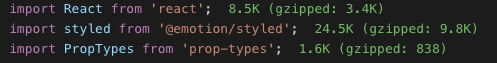
\includegraphics[width=\linewidth]{ReactInScope.png}
    \caption{React in scope}
    \label{fig:reactImport}
\end{figure}

\subsection{\IfLanguageName{dutch}{Pure component}{Pure component}}
\label{sec:pureComponent}

Pure component is exact hetzelfde als een gewoon component in React. Het verschil tussen beiden ligt hem in de lifecycle methode `shouldComponentUpdate()` die op een andere manier uitgevoerd wordt. Bij een normaal component zal er altijd een re-render uitgevoerd worden wanneer er iets aan props of state veranderd. In een pure component wordt er in shouldComponentUpdate shallow comparison gedaan van props en state.\\
Shallow comparison vergelijkt de waarden en referenties van de vorige props en state, met de volgende. Deze controle is goedkoop, zeker in vergelijking met het telkens re-renderen van een component. Het nadeel is dat er geen controle wordt gedaan voor de waarden in geneste objecten.\\
Een pure component gaat ervoor zorgen dat er minder re-renders gebeuren. Dit wordt ook overgedragen naar de kinderen van een pure component, daardoor is het af te raden om van componenten met kinderen pure components te maken.\\
\newline
Een component is best te veranderen naar een pure component wanneer het eenvoudige state en props bevat. Het gebruik van een pure component geeft een performantie boost zonder dat er veel aanpassingen moeten worden gedaan aan de intiële code. In figuur ~\ref{fig:extendPureComponent} wordt afgebeeld wat er moet worden veranderd om van een gewoon component een pure component te maken.

\begin{figure}[H]
    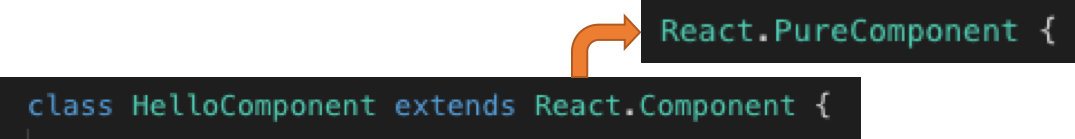
\includegraphics[width=\linewidth]{ExtendPureComponent.png}
    \caption{Changing component to pure component}
    \label{fig:extendPureComponent}
\end{figure}

\subsection{\IfLanguageName{dutch}{React Memo}{React Memo}}
\label{sec:memo}

Memo is gelijkaardig aan het pure component principe, waarbij het helpt om rendering te controleren. Memoization is een techniek voor het optimaliseren van snelheid in computer programma's. Door de dure functies, die regelmatig worden uitgevoerd, op te slaan in het cache geheugen kunnen ze veel sneller uitgevoerd worden in de toekomst. React memo werkt op hetzelfde principe.\\
Als een component wordt gewikkeld in `React.memo()` wordt bij elke re-render enkel de delen die een re-render nodig hebben opnieuw gerendert. De React.memo functie werkt voor functionele component als een extensie van React.PureComponent.

%=======================================================================
% Hooks sub hoofdstuk
%=======================================================================

\subsection{\IfLanguageName{dutch}{Hooks}{Hooks}}
\label{sec:hooks}

Hooks biedt alles wat een klasse component kan, voor een functioneel component. Vóór Reactv16.8 was het gebruik van functionele componenten voor de presentatie van domme en eenvoudige \gls{ui} elementen. De komst van hooks brengt een volledige \gls{api} voor functionele componenten met zich mee om te fungeren als klasse componenten.\\

\subsubsection{\IfLanguageName{dutch}{useState}{useState}}
\label{sec:useState}

-- Inhoud over useState binnen hooks --

\subsubsection{\IfLanguageName{dutch}{useEffect}{useEffect}}
\label{sec:useEffect}

-- Inhoud over useEffect binnen hooks --

\subsubsection{\IfLanguageName{dutch}{useCallback}{useCallback}}
\label{sec:useCallback}

-- Inhoud over useCallback binnen hooks --

%=======================================================================
% React concepten hoofdstuk
%=======================================================================

\section{\IfLanguageName{dutch}{React concepten}{React concepts}}

\subsection{\IfLanguageName{dutch}{Bundling}{Bundling}}
\label{sec:bundeling}

Bij het maken van een React applicatie wordt de gehele code base onderverdeeld in componenten en functionaliteiten van third party libraries. De code van die componenten en third party libraries wordt in andere delen van de applicatie geimporteerd. Hoe meer code dat componenten importeren, hoe groter en complexer ze worden. De kost om javaScript code te parsen en compilen is enorm. De laadtijd van webpagina's stijgt samen met het groter en complexer worden van componenten, omdat meer code geparsed en gecompiled moet worden.\\
Bundeling zorgt dat alle geimporteerde documenten opgehaald worden en in één bundel gestoken. De bundel wordt meegegeven aan de webpagina waarmee het de volledige applicatie kan inladen.  

\subsection{\IfLanguageName{dutch}{Code splitting}{Code splitting}}
\label{sec:codeSplitting}

Bundlers zoals Webpack en Browserify doen automatisch aan bundling. De meeste bundlers voorzien oplossingen voor de complicaties die bundling kan meebrengen in verband met laadtijden van webpagina's.\\
Code splitting is één van de oplossingen voor het controleren van bundle grootes in een applicatie. Het principe helpt door \gls{js} code te verdelen in stukken en enkel de delen die nodig zijn, voor de gebruiker, op een bepaald moment in te laden. Zo wordt met een minimum aan code waarde gecreëerd voor de \gls{ui}.\\




\subsection{\IfLanguageName{dutch}{React virtual DOM}{React virtual DOM}}
\label{ch:reactVirtualDOM}

-- Inleiding tot het hoofdstuk voor virtual DOM binnen React. --

\subsubsection{\IfLanguageName{dutch}{Wat is DOM?}{What is DOM?}}
\label{sec:watIsDOM}

Meer over het DOM (Data Object Model) van een browser en hoe er mee wordt gecommuniceerd. (JavaScript, compilers, ...)

\subsubsection{\IfLanguageName{dutch}{Virtual DOM}{Virtual DOM}}
\label{sec:virtualDOM}

% KLAD! Uses the render-diff process
% %%%%%%%%%%
Componenten worden geïnjecteerd met data en bevatten stukken van de UI die op basis van die data een bepaalde vorm aannemen. Enkel wanneer de data naar een component veranderd zal deze het stuk van de UI die hij beheert gaan aanpassen. React plaatst dan het geüpdatet component in de virtuele DOM boom, wat een kopie is van de werkelijke DOM boom in de browser, en vergelijkt het de reeds bestaande referentie van het component met de geüpdatet versie. Wanneer er verschillen zijn in structuur tussen de componenten zal er een update gedaan worden van het werkelijke component in het browser DOM.

\section{\IfLanguageName{dutch}{Tools}{Tools}}
\label{sec:toolsOplossingen}

\subsection{\IfLanguageName{dutch}{Webpack}{Webpack}}
\label{sec:webpack}

\subsection{\IfLanguageName{dutch}{Server side renderen}{Server side rendering}}
\label{sec:ssr}
            
